% Chapter 5

\chapter{Experimental Evaluation} % Main chapter title
\label{chap:Chapter5} % For referencing the chapter elsewhere, use \ref{chap:Chapter5}

%----------------------------------------------------------------------------------------

This chapter evaluates the system implemented in Chapter~\ref{chap:Chapter4}. It describes the experimental setup (Section~\ref{sec:eval_setup}), reports results for linguistic error detection (Section~\ref{sec:eval_ling}), mathematical error detection (Section~\ref{sec:eval_math}), and student profiling (Section~\ref{sec:eval_profile}), and closes with a discussion of the hypotheses, limitations, and threats to validity (Section~\ref{sec:eval_discuss}). All reported numbers come from the final training and evaluation runs; intermediate results that were later superseded (or found to be artifacts) are reported only where they carry a methodological lesson, and are labeled as such.

\section{Experimental Setup}
\label{sec:eval_setup}

Every evaluation in this chapter shares one experimental design. It consists of the experimental research questions, the datasets, the metrics, and the implementation details that are needed to reproduce the results.

\subsection{Research Questions}
\label{sec:eval_setup_rq}

The experiments operationalize the thesis hypotheses through four experimental questions, numbered RQ1--RQ4 independently of the research questions Q1--Q5 of Chapter~\ref{chap:introduction}; the corresponding hypothesis or question is given in parentheses:

\begin{itemize}
    \item RQ1 (H1): How accurately do the detection modules identify and classify difficulty-linked error patterns in student responses, including on text from the target population?
    \item RQ2 (H2): Does synthetic data improve detection performance on \emph{real} data, compared to training on scarce real data alone?
    \item RQ3 (Q3): How do symbolic malrule detection and a simple ML classifier compare on arithmetic procedural bugs, in accuracy and in robustness?
    \item RQ4 (H3): Does unsupervised clustering of aggregated errors yield difficulty profiles that are recoverable (simulation), real (archetype shapes in real data), and stable (longitudinal real data)?
\end{itemize}

\subsection{Datasets}
\label{sec:eval_setup_data}

Table~\ref{tab:eval_datasets} summarizes all datasets. The linguistic training pool combines rule-based synthetic corruptions with two public GEC corpora converted through the taxonomy mapper (Section~\ref{sec:impl_ling_data}); the two benchmark sets are entirely held out. For mathematics, both methods are trained/matched on generated malrule data. For profiling, the simulated students are complemented by two real datasets.

\begin{table}[h]
\centering
\caption[Datasets used in the evaluation.]{Datasets used in the evaluation. ``In-scope'' sentences contain at least one error belonging to the thesis taxonomy. Holbrook: 531 of the 1{,}254 parsed sentences contain an in-scope error and form the BIO benchmark; the per-student profiles of Sections~\ref{sec:eval_profile_holbrook} and~\ref{sec:eval_profile_fidelity} use all 1{,}254 (error density requires the error-free sentences).}
\label{tab:eval_datasets}
\small\setlength{\tabcolsep}{4pt}
\begin{tabular}{@{}llr>{\raggedright\arraybackslash}p{0.27\textwidth}@{}}
\toprule
\textbf{Module} & \textbf{Dataset} & \textbf{Size} & \textbf{Role} \\
\midrule
Linguistic & Synthetic corruptions & 1{,}000{,}000 sent. & train (90\%) / eval (10\%) \\
Linguistic & BEA-2019 W\&I+LOCNESS & 2{,}584 sent. & real pool: train/eval (90/10) \\
Linguistic & CLC FCE v2.1 (train+dev) & 4{,}331 sent. & real pool: train/eval (90/10) \\
Linguistic & CLC FCE v2.1 (test) & 383 sent. & held-out benchmark \\
Linguistic & Holbrook (struggling children) & 531 sent. & held-out, domain shift \\
Math & Generated malrule problems & $2\times10^6$ & train (70\%) / test (30\%, stratified) \\
Profiling & Simulated students & 180 students/run & archetype recovery \\
Profiling & Holbrook per-student profiles & 19 students & real archetype shapes \\
Profiling & ASSISTments 2009--10 & 525{,}534 resp. & real longitudinal stability \\
\bottomrule
\end{tabular}
\end{table}

\subsection{Metrics}
\label{sec:eval_setup_metrics}

Linguistic detection is scored with strict span-level precision, recall, and $F_1$ (seqeval): a predicted span counts as correct only if its boundaries and error type both match the gold span. Mathematical detection reports accuracy and macro-$F_1$ over the malrule classes. Clustering is scored with the silhouette coefficient \parencite{Rousseeuw1987} for internal quality and the Adjusted Rand Index \parencite{HubertArabie1985} against ground truth (simulation) or between independent re-clusterings (stability).

\subsection{Implementation Details}
\label{sec:eval_setup_impl}

Neural training ran on a single NVIDIA RTX 5070 (12\,GB VRAM) in fp32 (Section~\ref{sec:impl_ling_training}), with learning rate $2\times10^{-5}$, 10\% warmup, batch size 16, sequence length 64, and 2/8/2 epochs for curriculum stages 1/2/3 respectively (epoch counts scaled inversely with each stage's dataset growth). Wall-clock times were approximately 1.9\,h for each of stages 1 and 3 (the 1M-example stages) and under 4 minutes for stage 2. All random seeds are fixed; every reported evaluation is reproducible from serialized run summaries. The NaN-parameter audit passed after every stage (zero corrupted tensors).

\section{Linguistic Error Detection Results}
\label{sec:eval_ling}

The linguistic module is evaluated in five steps: each curriculum stage on its own split, the benchmarks on real data, a comparison with baselines that adds bootstrap confidence intervals, the effect of synthetic data volume versus domain match, and finally a real-only baseline trained from scratch. That last baseline is the reference for judging the value of synthetic data.

\subsection{Curriculum Stages}
\label{sec:eval_ling_stages}

Table~\ref{tab:ling_stages} reports each curriculum stage on its own evaluation split. Two of these numbers need careful reading, and the reasons are themselves findings about evaluation design.

\begin{table}[h]
\centering
\caption[Three-stage curriculum results (span-level, seqeval).]{Three-stage curriculum results (span-level, seqeval). Each stage is evaluated on its own held-out split; the compositions differ, so stages are not directly comparable to each other in this table (see text and Table~\ref{tab:ling_real}).}
\label{tab:ling_stages}
\small\setlength{\tabcolsep}{4pt}
\begin{tabular}{llccc}
\toprule
\textbf{Stage} & \textbf{Eval split} & \textbf{Precision} & \textbf{Recall} & \textbf{$F_1$} \\
\midrule
1: synthetic only & synthetic (100k) & 0.986 & 0.993 & 0.990 \\
2: real fine-tuning (from stage 1) & real (692) & 0.558 & 0.648 & 0.600 \\
3: combined & synth.+real (99.3\% synth.) & 0.986 & 0.990 & 0.988 \\
\bottomrule
\end{tabular}
\end{table}

Stage 1's high score is legitimate generalization over the corruption distribution (the evaluation sentences' base texts never appear in training), but it measures performance on synthetic error patterns, not real ones. (An earlier run with only 20 template base sentences scored a perfect 1.0 here; that was pure memorization and prompted the 600{,}000-sentence base pool.) Stage 3's aggregate score is dominated by the synthetic 99.3\% of its evaluation split and therefore does not answer any question about real data. The stage-2 score ($F_1 = 0.600$ on real learner text) is the real-data reference for measuring the marginal value of the combined stage~3. It is not a real-only baseline: stage 2 is initialized from the synthetic stage-1 checkpoint (Section~\ref{sec:impl_ling_training}). The real-only baseline, trained from scratch on the real pool alone, is reported in Section~\ref{sec:eval_ling_scratch}.

\subsection{Real-Data Benchmarks}
\label{sec:eval_ling_real}

Table~\ref{tab:ling_real} evaluates the final (stage-3) model on three all-real benchmarks: the same real evaluation split used by stage 2 (enabling a direct comparison), the held-out FCE test set (same domain, never seen), and the Holbrook set (domain shift to the target population).

\begin{table}[h]
\centering
\caption{Final model on all-real benchmarks (span-level, seqeval).}
\label{tab:ling_real}
\small
\begin{tabular}{@{}>{\raggedright\arraybackslash}p{0.44\textwidth}rccc@{}}
\toprule
\textbf{Benchmark} & \textbf{Sent.} & \textbf{Precision} & \textbf{Recall} & \textbf{$F_1$} \\
\midrule
Real eval split (= stage-2 split) & 692 & 0.607 & 0.681 & \textbf{0.642} \\
FCE test (held out, same domain) & 383 & 0.561 & 0.630 & 0.594 \\
Holbrook (held out, domain shift) & 531 & 0.392 & 0.402 & 0.397 \\
\midrule
\emph{Reference:} stage-2 checkpoint (synthetic$\to$real), same real split & 692 & 0.558 & 0.648 & 0.600 \\
\bottomrule
\end{tabular}
\end{table}

Three results stand out:

\begin{enumerate}
    \item The combined stage adds little over stage 2 in this seed. On the identical real evaluation split, the final model reaches $F_1 = 0.642$ versus $0.600$ for the stage-2 checkpoint, a $+4.2$-point difference that comes mainly from precision ($0.558 \rightarrow 0.607$). This difference is from a single seed; the multi-seed analysis in Section~\ref{sec:eval_ling_scale} shows it is not stable across seeds (paired intervals straddle zero). This comparison does not test H2, since both models were pre-trained on synthetic data; the comparison against real-only training is in Section~\ref{sec:eval_ling_scratch}.
    \item The absolute performance level is consistent on a fully held-out set. The FCE test result ($0.594$) is close to the real-split result, which suggests that the level of performance is not an artifact of the particular 90/10 split.
    \item Domain shift to the target population is the dominant limitation. On the Holbrook benchmark (real writing by children with literacy difficulties), $F_1$ drops to $0.397$, roughly 20 points below same-domain performance. The error pattern is diagnostic: the model over-predicts phonological spans (574 predicted vs.\ 436 gold \texttt{B-PHONO}) and under-predicts orthographic ones (356 vs.\ 568 gold \texttt{B-ORTHO}). Adult L2 learners and struggling child writers make errors with different type distributions, and a detector trained on the former does not fully transfer to the latter. This quantifies, on the thesis's own target population, the data-scarcity problem that motivates H2, and it marks in-domain data as the most valuable direction for future work (Chapter~6).
\end{enumerate}

\subsection{Baseline Comparison and Statistical Robustness}
\label{sec:eval_ling_baseline}

Two additions give the neural numbers a floor and a confidence interval. First, a non-neural baseline: an off-the-shelf dictionary spell-checker whose flagged tokens (and suggested corrections) are routed through the same taxonomy mapper, with hypo-/hypersegmentation checks for SEG; it is the strongest simple system assemblable from standard parts. Second, 95\% bootstrap confidence intervals (2{,}000 sentence-level resamples), with the neural-vs-baseline difference computed \emph{paired} on identical resamples. Table~\ref{tab:ling_baseline_ci} reports both on the two held-out benchmarks. (Scoring here is word-level span matching, since the baseline has no subword structure; the neural point estimates therefore differ slightly from the subword-level protocol of Table~\ref{tab:ling_real} (FCE $0.669$ word-level vs.\ $0.594$ subword-level), without affecting any comparison within either table.)

\begin{table}[h]
\centering
\caption[Neural model vs.\ spell-checker baseline, word-level span $F_1$ with 95\% bootstrap CIs.]{Neural model vs.\ spell-checker baseline, word-level span $F_1$ with 95\% bootstrap CIs (2{,}000 resamples; difference paired on identical resamples).}
\label{tab:ling_baseline_ci}
\begin{tabular}{lccc}
\toprule
\textbf{Benchmark} & \textbf{Baseline} & \textbf{Neural} & \textbf{$\Delta$ (paired)} \\
\midrule
FCE test & 0.459 [0.419, 0.499] & 0.669 [0.628, 0.709] & $+0.210$ [0.156, 0.264] \\
Holbrook & 0.318 [0.286, 0.348] & 0.403 [0.372, 0.434] & $+0.084$ [0.034, 0.132] \\
\bottomrule
\end{tabular}
\end{table}

Three observations. The neural model beats the baseline decisively in its training domain ($+21$ points, CI excluding zero by a wide margin) and still significantly under domain shift ($+8.4$ points, CI $[0.034, 0.132]$). The baseline also degrades sharply on Holbrook (0.459 $\rightarrow$ 0.318), which shows that part of the difficulty is intrinsic to the population's writing (denser, less conventional errors) and cannot be attributed solely to the neural model's training distribution. The intervals confirm that the neural-versus-baseline advantage does not rest on resampling noise; the same cannot be said of the stage-2-versus-final difference, as the next section shows.

\subsection{Synthetic Scale: Volume versus Domain Match}
\label{sec:eval_ling_scale}

Section~\ref{sec:eval_ling_real} leaves open whether synthetic pre-training helps on real data at all; a related, design-relevant question is whether more synthetic data helps. The synthetic corpus is generated and can therefore be made arbitrarily large, so the answer matters for practice: if real-data performance scales with synthetic volume, the cheapest lever is to generate more; if it does not, effort is better spent elsewhere. To test this, the identical three-stage curriculum was retrained with the synthetic pool capped at three volumes spanning two orders of magnitude ($10^4$, $10^5$, $10^6$ examples), holding the real corpus, architecture, hyperparameters, and random seed fixed. Each resulting model was scored on two held-out splits: its own in-domain synthetic split (which grows with the pool) and the same real evaluation split used for the H2 comparison ($n = 692$). Scoring here follows the word-level span protocol of Table~\ref{tab:ling_baseline_ci} (first-subtoken alignment), so these numbers are directly comparable to the paired-CI analysis and run a few points above the subword-level figures of Table~\ref{tab:ling_real}.

\begin{table}[h]
\centering
\caption[Synthetic-scale ablation (word-level span $F_1$, seqeval).]{Synthetic-scale ablation (word-level span $F_1$, seqeval). Same real held-out split ($n=692$) as the H2 comparison; single seed per row. In-domain and real-domain $F_1$ move in opposite directions.}
\label{tab:ling_scale}
\begin{tabular}{rcccc}
\toprule
\textbf{Synthetic examples} & \textbf{In-domain $F_1$} & \textbf{Real $F_1$} & \textbf{Real precision} & \textbf{Real recall} \\
\midrule
$10^4$ (10k)   & 0.934 & \textbf{0.729} & 0.706 & 0.754 \\
$10^5$ (100k)  & 0.979 & 0.710 & 0.687 & 0.735 \\
$10^6$ (1M)    & 0.992 & 0.697 & 0.674 & 0.723 \\
\bottomrule
\end{tabular}
\end{table}

The two columns form a scissors (Figure~\ref{fig:scale_ablation}). Scaling the synthetic pool $100\times$ improves in-domain $F_1$ monotonically ($0.934 \rightarrow 0.992$, $+5.9$ points) while real-domain $F_1$ falls monotonically ($0.729 \rightarrow 0.697$, $-3.2$ points). The best real-data model is the one trained on the least synthetic data, and its real $F_1$ of $0.729$ is the highest of the three pools in this single-seed ablation. A plausible explanation is that additional synthetic examples fit the corruption distribution ever more tightly, and that this distribution differs systematically from real learner error, so a tighter fit to it transfers slightly worse. Under this reading, synthetic volume is not the bottleneck; the match between the synthetic error distribution and the target one is.

\begin{figure}[ht]
\centering
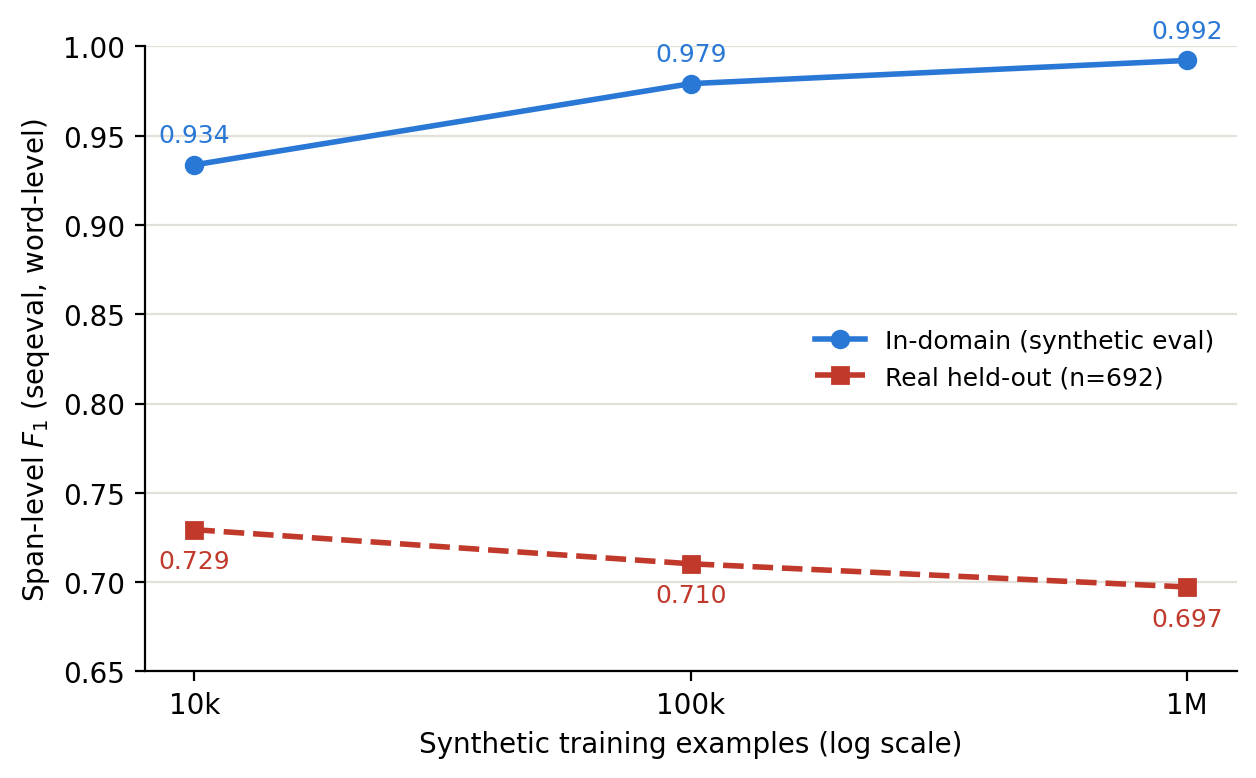
\includegraphics[width=0.8\textwidth]{figures/synthetic_scale_ablation.png}
\caption{Synthetic-scale ablation. In-domain $F_1$ rises with synthetic volume while real held-out $F_1$ falls: more synthetic data fits the corruption distribution more tightly at a small cost to real-data transfer.}
\label{fig:scale_ablation}
\end{figure}

This result should be read with two cautions. First, each row is a single seed, and the real-$F_1$ spread across the whole sweep ($0.032$) is of the same order as the bootstrap confidence intervals in Table~\ref{tab:ling_baseline_ci}; no single pairwise gap is individually significant, and a consistently ordered three-point trend is suggestive but not conclusive (under pure noise, any particular ordering of three points has probability $1/6$). What lends the pattern credibility is that it runs opposite to the in-domain trend, and that it is corroborated by the multi-seed analyses below and by the real-only-from-scratch comparison of Section~\ref{sec:eval_ling_scratch}. Second, the stage-2-versus-final difference of Section~\ref{sec:eval_ling_real} was re-examined in a multi-seed paired analysis (Table~\ref{tab:ling_multiseed}). For each of three additional seeds, the stage-2 checkpoint and the final curriculum model were compared on identical bootstrap resamples of the evaluation set. At the headline synthetic pool, the paired differences on the real split are $+0.016$, $-0.011$, and $+0.003$. The curriculum was then retrained at the ablation-optimal $10^4$ pool for the same three seeds and evaluated both on the real split and on the FCE test set; because the real split was itself used to select that scale, a positive result there would only be suggestive, whereas FCE was never consulted during scale selection and is the independent confirmation set. All nine 95\% intervals straddle zero, and at the $10^4$ scale the mean paired difference is in fact slightly negative ($-0.008$ real, $-0.005$ FCE): even at the synthetic volume most favorable to real-data transfer, and even on the split that chose it, the combined stage~3 yields no reliable paired gain over the stage-2 checkpoint. The single-seed $+4.2$-point difference of Section~\ref{sec:eval_ling_real} is therefore best read as the favorable end of a distribution centered near zero, not as a stable effect. What this comparison cannot show is whether the synthetic stages help relative to training on real data alone, because both checkpoints share the synthetic stage~1. That question, the one H2 poses, is addressed next.

\begin{table}[ht]
\centering
\caption[Multi-seed paired comparison of the stage-2 checkpoint against the full curriculum model.]{Multi-seed paired comparison of the stage-2 checkpoint (synthetic pre-training followed by real fine-tuning) against the full curriculum model (final), word-level span $F_1$ with paired bootstrap 95\% intervals (2{,}000 sentence resamples). Real split $n=692$; FCE test $n=383$. The real split was used to select the $10^4$ scale; FCE was not, making it the independent confirmation set. Every interval straddles zero.}
\label{tab:ling_multiseed}
\begin{tabular}{llccccc}
\toprule
\textbf{Synthetic pool} & \textbf{Eval set} & \textbf{Seed} & \textbf{Stage-2 $F_1$} & \textbf{Final $F_1$} & \textbf{$\Delta$} & \textbf{95\% CI} \\
\midrule
$10^6$ & real & 1 & 0.681 & 0.696 & $+0.016$ & $[-0.009, 0.039]$ \\
$10^6$ & real & 2 & 0.703 & 0.693 & $-0.011$ & $[-0.035, 0.014]$ \\
$10^6$ & real & 3 & 0.663 & 0.666 & $+0.003$ & $[-0.022, 0.029]$ \\
\midrule
$10^4$ & real & 1 & 0.730 & 0.722 & $-0.008$ & $[-0.025, 0.010]$ \\
$10^4$ & real & 2 & 0.728 & 0.714 & $-0.014$ & $[-0.033, 0.004]$ \\
$10^4$ & real & 3 & 0.690 & 0.689 & $-0.001$ & $[-0.020, 0.018]$ \\
\midrule
$10^4$ & FCE  & 1 & 0.687 & 0.679 & $-0.008$ & $[-0.034, 0.018]$ \\
$10^4$ & FCE  & 2 & 0.703 & 0.691 & $-0.012$ & $[-0.036, 0.012]$ \\
$10^4$ & FCE  & 3 & 0.683 & 0.688 & $+0.006$ & $[-0.020, 0.031]$ \\
\bottomrule
\end{tabular}
\end{table}

\subsection{Real-Only Baseline Trained From Scratch}
\label{sec:eval_ling_scratch}

The comparisons above all involve models that were pre-trained on synthetic data: the stage-2 checkpoint is the stage-1 synthetic model fine-tuned on real data (Section~\ref{sec:impl_ling_training}), so stage-2-versus-final measures only the marginal value of the combined stage~3. H2 asks whether synthetic pre-training helps relative to training on the scarce real data alone, and answering that requires a baseline with no synthetic stage. This baseline was trained for four seeds and compared against the curriculum at both the headline $10^6$ pool and the ablation-optimal $10^4$ pool (seeds 1--3, the seeds for which $10^4$ curriculum models exist; Table~\ref{tab:ling_multiseed}): DeBERTa-v3-base initialized from the public pretrained checkpoint and fine-tuned on the real training pool only, under exactly the stage-2 configuration (8 epochs, learning rate $2\times10^{-5}$, 10\% warmup, gradient clipping at 1.0, batch size 16, fp32, focal loss with the same class weights). For each seed, the real 90/10 split is the same one used by the curriculum run with that seed, so the real-only model and each curriculum model are compared on identical evaluation sentences, with the difference computed paired on 2{,}000 sentence-level bootstrap resamples under the word-level span protocol of Table~\ref{tab:ling_baseline_ci}.

\begin{table}[ht]
\centering
\caption[Real-only training from scratch versus the synthetic-to-real curriculum.]{Real-only training from scratch (no synthetic stage) versus the synthetic-to-real curriculum at the headline ($10^6$) and the ablation-optimal ($10^4$) synthetic pools, word-level span $F_1$ on the identical real evaluation split ($n=692$) for each seed, with paired bootstrap 95\% intervals (2{,}000 resamples). $\Delta$ = curriculum $-$ real-only; negative values favor real-only training. No $10^4$ curriculum model exists for seed 0.}
\label{tab:ling_scratch}
\small\setlength{\tabcolsep}{4pt}
\begin{tabular}{ccccccc}
\toprule
\textbf{Synthetic pool} & \textbf{Seed} & \textbf{Real-only $F_1$} & \textbf{Curriculum $F_1$} & \textbf{$\Delta$} & \textbf{95\% CI} & \textbf{$P(\Delta \leq 0)$} \\
\midrule
$10^6$ & 0 & 0.729 & 0.692 & $-0.037$ & $[-0.070, -0.004]$ & 0.983 \\
$10^6$ & 1 & 0.721 & 0.696 & $-0.025$ & $[-0.054, +0.003]$ & 0.958 \\
$10^6$ & 2 & 0.725 & 0.693 & $-0.032$ & $[-0.064, -0.001]$ & 0.978 \\
$10^6$ & 3 & 0.736 & 0.666 & $-0.070$ & $[-0.105, -0.034]$ & 1.000 \\
\midrule
$10^4$ & 1 & 0.721 & 0.722 & $+0.001$ & $[-0.025, +0.025]$ & 0.480 \\
$10^4$ & 2 & 0.725 & 0.714 & $-0.011$ & $[-0.034, +0.011]$ & 0.839 \\
$10^4$ & 3 & 0.736 & 0.689 & $-0.047$ & $[-0.077, -0.016]$ & 1.000 \\
\bottomrule
\end{tabular}
\end{table}

At the headline pool the result (Table~\ref{tab:ling_scratch}) is unambiguous in direction: in every seed, the model trained on the real training split alone (the 6{,}915-sentence pool minus the 692 held-out evaluation sentences) outperforms the full $10^6$ curriculum by 2.5 to 7.0 $F_1$ points, and in three of the four seeds the paired 95\% interval excludes zero. At that volume, synthetic pre-training does not improve real-data detection; it lowers it. This is consistent with the scale ablation (real-data $F_1$ falling as synthetic volume grows) and with the null stage-2-versus-final differences: the synthetic stages move the model toward the corruption distribution, and subsequent real fine-tuning does not fully recover from that.

At the ablation-optimal $10^4$ pool the penalty shrinks but no gain appears: the paired differences are $+0.001$, $-0.011$ and $-0.047$, with two intervals straddling zero and one (seed 3) excluding it on the negative side. The most favorable reading is that a small synthetic pool is, in two of three seeds, statistically indistinguishable from real-only training; in no seed does the curriculum reliably exceed it. Taken together with the $10^6$ rows, the picture is a dose-response one: the more synthetic data precedes real fine-tuning, the further the model ends up below the real-only reference.

Two caveats bound the reading. First, the $10^4$ comparison rests on three seeds, one of which is an outlier in the negative direction; more seeds would tighten the parity claim. Second, the real-only models are evaluated in their training domain; whether synthetic pre-training helps or hurts under domain shift (Holbrook) was not tested from scratch. Within these bounds, H2 is not supported at either evaluated volume (Section~\ref{sec:eval_discuss_hyp}).

\section{Mathematical Error Detection Results}
\label{sec:eval_math}

The mathematical module is evaluated by comparing exact symbolic simulation with the feature-based classifier on three questions. The first is how each method does on clean answers that follow the modeled malrules. The second is how each holds up when those answers are perturbed. The third is how the design of a diagnostic item decides whether different misconceptions can be told apart.

\subsection{Clean Malrule Answers}
\label{sec:eval_math_clean}

On the held-out, stratified 30\% test split of the 1{,}000{,}000 generated problems per operation family, whose incorrect answers follow modeled malrules exactly (ambiguous SFL/BORROW\_NO\_DEC collisions filtered; Section~\ref{sec:impl_math_malrule}), both methods are near-ceiling: the symbolic detector achieves accuracy $1.000$ and the gradient-boosted classifier accuracy $0.997$ (macro-$F_1$ $0.800$ and $0.797$ respectively; the gap between macro-$F_1$ and accuracy is an artifact of including the \texttt{OTHER\_ERROR} class, which never occurs in this test set, in the macro average with a score of zero, not a property of the methods). On answers that exactly follow a known buggy procedure, exact simulation is unbeatable by construction, and the classifier nearly matches it. Both figures characterize correctness under the modeled synthetic conditions, not diagnostic accuracy on real student work, which was not evaluated.

\subsection{Robustness Under Perturbation}
\label{sec:eval_math_noise}

The methods separate sharply under realistic noise. When a $\pm 1$ digit slip is added to each malrule answer, which models a student who applies a buggy procedure and also makes an incidental arithmetic error, the symbolic detector's accuracy collapses to $0.0$ (it requires exact matches by construction), while the ML classifier retains $61.7\%$ accuracy. This is the main precision-versus-robustness trade-off for RQ3: symbolic malrule detection offers exactness and interpretability but has zero tolerance to deviation, while a simple feature-based classifier degrades gracefully. A deployed system should treat them as complements. Exact matches yield high-confidence, interpretable diagnoses, and the classifier is a fallback for answers where no malrule matches exactly.

\subsection{Diagnostic Item Design: Malrule Distinguishability}
\label{sec:eval_math_distinguish}

A third experiment generalizes an incidental finding from dataset generation (Section~\ref{sec:impl_math_malrule}): whether a misconception can be identified from an answer at all depends on the structure of the problem posed. For each problem structure (operand digit count, with and without forcing a borrow-through-zero), 5{,}000 problems were generated and every malrule's simulated answer compared against all others'. Table~\ref{tab:distinguish} reports the fraction of problems on which all three subtraction malrules produce mutually distinct answers (also distinct from the correct one), that is, problems that can in principle diagnose any of the three misconceptions from a single answer.

\begin{table}[h]
\centering
\caption[Malrule distinguishability by problem structure (5{,}000 generated problems per cell).]{Malrule distinguishability by problem structure (5{,}000 generated problems per cell). ``All 3 distinct'' = SFL, BORROW\_ZERO and BORROW\_NO\_DEC yield pairwise different answers, all different from the correct answer.}
\label{tab:distinguish}
\begin{tabular}{ccccc}
\toprule
\textbf{Digits} & \textbf{Zero-borrow forced} & \textbf{All 3 distinct} & \textbf{SFL unique} & \textbf{SFL$=$BND collisions} \\
\midrule
2 & no  & 0.0\%  & 88.5\% & 11.5\% \\
3 & no  & 4.8\%  & 91.7\% & 8.3\% \\
4 & no  & 14.0\% & 93.4\% & 6.6\% \\
6 & no  & 30.7\% & 96.8\% & 3.2\% \\
2 & yes & 0.0\%  & 88.9\% & 11.1\% \\
4 & yes & 43.5\% & 95.5\% & 4.5\% \\
6 & yes & 74.8\% & 98.4\% & 1.6\% \\
\bottomrule
\end{tabular}
\end{table}

The main result is that two-digit problems can never distinguish all three misconceptions (0\% in both conditions; BORROW\_ZERO is never uniquely identifiable at two digits), while six-digit problems with a forced borrow-through-zero distinguish all three on 74.8\% of items. Distinguishability rises monotonically with digit count, and forcing a zero in the borrow chain raises it about three times at four digits ($14.0\% \rightarrow 43.5\%$) and about 2.4 times at six digits ($30.7\% \rightarrow 74.8\%$). The practical implication is a change of question. Besides asking ``how good is the detector?'', a diagnostic system should ask ``which problems make the misconceptions detectable?'' Item difficulty (more digits, zeros in the minuend) is not an obstacle to diagnosis but a prerequisite for it. This gives the system a concrete item-selection policy for deployment, and it connects to the classical observation that bug diagnosis requires adequately discriminating test items \parencite{VanLehn1990}.

\section{Student Profiling Results}
\label{sec:eval_profile}

Four experiments evaluate the profiling module. The first tests, in simulation, how well known archetypes are recovered as separability and data volume change. The second looks for archetype-like structure in real writing by children (Holbrook), and the third for longitudinal stability of behavioral profiles in real data (ASSISTments). The fourth measures the fidelity of the profiles under domain shift, comparing open-world and closed-world settings.

\subsection{Archetype Recovery: Separability $\times$ Data Volume}
\label{sec:eval_profile_ari}

Figure~\ref{fig:ari_sweep} reports the two-factor simulation experiment: Adjusted Rand Index of KMeans archetype recovery as a function of archetype dominance $d$ (how concentrated each profile's error mass is on its characteristic error types) and total observations per student, averaged over three seeds (180 simulated students, six archetypes).

\begin{figure}[ht]
\centering
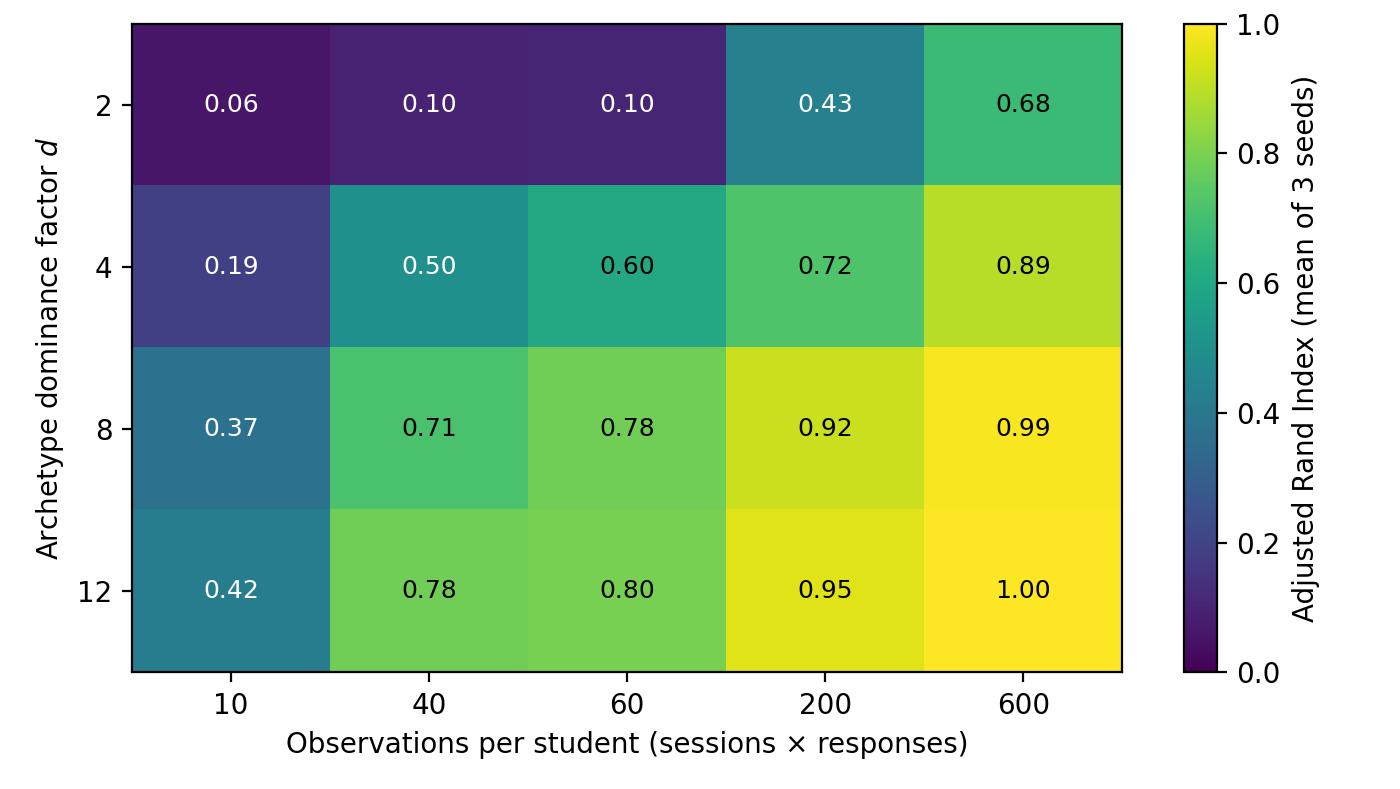
\includegraphics[width=0.85\textwidth]{figures/ari_sweep_heatmap.png}
\caption{Archetype recovery (ARI, mean of 3 seeds) as a function of profile separability ($d$) and observations per student. Recovery requires both factors: neither strong separability with little data nor abundant data on weakly-separated profiles suffices.}
\label{fig:ari_sweep}
\end{figure}

The pattern is monotone in both factors but strongly interactive. With weakly separated profiles ($d=2$), even 600 observations per student reach only ARI $0.68$; with sharply separated profiles ($d \geq 8$), 200 observations suffice for ARI $> 0.9$, and recovery is close to perfect at 600. At realistic classroom volumes (tens of responses per student), only strongly distinct profiles are recoverable at all (ARI $0.37$--$0.78$ at 10--60 observations for $d \geq 8$). For deployment, this means that a system of this kind needs on the order of a few hundred labeled responses per student before its profile clusters can be trusted, unless the underlying difficulty profiles are already sharply distinct.

\subsection{Real Archetype Shapes (Holbrook)}
\label{sec:eval_profile_holbrook}

Clustering the 19 real per-student error distributions from the Holbrook corpus (error-type proportions plus error density) yields an optimal $k=3$ (silhouette $0.338$) with clearly interpretable centroids:

\begin{table}[h]
\centering
\caption{Real per-student clusters in the Holbrook corpus ($k=3$).}
\label{tab:holbrook_clusters}
\begin{tabular}{lrcccc}
\toprule
\textbf{Cluster} & \textbf{n} & \textbf{PHONO} & \textbf{ORTHO} & \textbf{SEG} & \textbf{Err.\ density} \\
\midrule
Mild, segmentation-leaning & 6 & 0.34 & 0.49 & 0.17 & 0.023 \\
Orthographic-dominant, high density & 8 & 0.34 & 0.60 & 0.05 & 0.060 \\
Phonological-dominant, high density & 5 & 0.56 & 0.38 & 0.06 & 0.071 \\
\bottomrule
\end{tabular}
\end{table}

Although $n=19$ permits no strong statistical claims, the qualitative finding matters for H3's plausibility: real struggling writers differ systematically in which error type dominates as well as in how many errors they make. In particular, a phonologically-dominant profile, the signature most associated with phonological-deficit accounts of dyslexia \parencite{ShaywitzShaywitz2005}, emerges from unsupervised clustering of real data without being assumed, under the Metaphone-based operationalization of the PHONO/ORTHO boundary (Section~\ref{sec:impl_ling_taxmap}). The derived centroids were exported in a form directly usable as simulation archetype weights; the ARI sweep of Section~\ref{sec:eval_profile_ari}, however, was run with the hand-specified archetypes, so replacing them with the real-data-derived weights is still a next step.

\subsection{Real Longitudinal Stability (ASSISTments)}
\label{sec:eval_profile_assistments}

For the 1{,}519 ASSISTments students with at least 50 responses, clustering per-student behavioral features finds an optimal $k=2$ (silhouette $0.385$) with a clean pedagogical reading:

\begin{table}[h]
\centering
\caption{Behavioral clusters in ASSISTments 2009--10 ($k=2$, raw-feature centroids).}
\label{tab:assistments_clusters}
\begin{tabular}{lcc}
\toprule
\textbf{Feature} & \textbf{``Coping'' (n=1{,}033)} & \textbf{``Struggling'' (n=486)} \\
\midrule
Accuracy & 0.719 & 0.411 \\
Mean attempts per problem & 1.38 & 2.22 \\
Hint-request rate & 0.104 & 0.355 \\
Median first-response time (s) & 25.0 & 16.2 \\
Repeated-failure rate ($\geq 3$ attempts) & 0.069 & 0.156 \\
\bottomrule
\end{tabular}
\end{table}

The struggling cluster answers faster, not slower. This is consistent with impulsive guessing and hint-fishing, a known behavioral signature in the educational data mining literature \parencite{BakerYacef2009}, and not with slow effortful work. The split-half stability test (Section~\ref{sec:impl_profile_real}) yields ARI $= 0.587$ between clusters computed independently from each student's odd- and even-indexed responses. Profile membership is therefore substantially, though not perfectly, stable across independent halves of a student's real history. Difficulty profiles behave as per-student traits with measurable noise, which is the regime in which the ARI sweep says a few hundred observations are needed for reliable clustering.

\subsection{Profile Fidelity Under Domain Shift: Open vs.\ Closed World}
\label{sec:eval_profile_fidelity}

The final experiment connects the linguistic domain gap (Section~\ref{sec:eval_ling_real}) to its downstream consequence for profiling, and quantifies what the screening mode (Sections~\ref{sec:method_models_screening} and~\ref{sec:impl_prototype_screening}) recovers. For each of the 19 Holbrook students, two error-type distributions over \{PHONO, ORTHO, SEG\} were built from the same 1{,}254 parsed sentences (all of each child's sentences, including the error-free ones; the 531-sentence BIO benchmark is the in-scope-error subset): a \emph{closed-world} profile from the target-known, deterministically mapped labels (what screening would produce), and an \emph{open-world} profile from the neural model's free-text detections.

The two profiles agree grossly in shape (mean cosine similarity $0.882$) but the aggregate hides the failure that matters most pedagogically. Ranking students, which is what a teacher's attention allocation uses, survives for error volume but not for error type: the Spearman rank correlation between open- and closed-world student orderings is $0.898$ for overall error density, but only $0.311$ for the PHONO proportion, $0.179$ for ORTHO, and $0.618$ for SEG. Under domain shift, the open-world detector still identifies almost perfectly which students err a lot, but it largely loses in which way they err, and the error-type mix is what distinguishes difficulty profiles from generic low performance.

This result completes the argument for the two-regime design: passive monitoring remains reliable for volume-based signals and same-domain deployments, while type-resolved profiling of the target population should be grounded in closed-world screening. Screening needs no model inference and so is not subject to training-population shift by construction, though it remains dependent on the mapper's operationalization and on the item bank.

\section{Discussion}
\label{sec:eval_discuss}

The results above are interpreted here in three parts. The hypotheses of Chapter~\ref{chap:introduction} are checked against the evidence, the findings are set against prior work, and the limitations and threats to validity that bound the conclusions are discussed.

\subsection{Hypotheses Revisited}
\label{sec:eval_discuss_hyp}

\textbf{H1} (detection of pedagogically meaningful errors): supported in its testable part, with a quantified domain gap. The mathematical module identifies modeled procedural bugs almost perfectly on clean generated answers, and the linguistic module reaches span-level $F_1 = 0.642$ on real learner text, a demanding metric (exact span and type). However, transfer to the target population is partial ($F_1 = 0.397$ on Holbrook), and the direction of its errors (over-flagging phonological, under-flagging orthographic spans) is itself interpretable in terms of the taxonomy. The part of H1 that refers to consistency with expert teacher annotations was not tested: no teacher-annotation or inter-annotator study was conducted, and performance is measured against the expert-produced gold annotations of the public corpora. ``Pedagogically meaningful'' is therefore supported in the sense that the detected categories are those of an instructionally grounded taxonomy, not in the sense of validated teacher agreement.

\textbf{H2} (synthetic data mitigates scarcity): not supported. Three lines of evidence converge. The direct test, real-only training from scratch versus the curriculum on identical real evaluation sentences with a paired bootstrap, shows the $10^6$ curriculum below real-only training in every one of four seeds, by 2.5 to 7.0 $F_1$ points, with three of four intervals excluding zero; at the $10^4$ pool the curriculum matches real-only training in two of three seeds and falls significantly below it in the third, never exceeding it (Table~\ref{tab:ling_scratch}). The scale ablation shows real-data performance declining as synthetic volume grows ($0.729 \rightarrow 0.697$ over $10^4 \rightarrow 10^6$), the opposite of the in-domain trend (Table~\ref{tab:ling_scale}). And the nine paired stage-2-versus-final comparisons are centered near zero (Table~\ref{tab:ling_multiseed}), so the combined stage does not compensate. The reading supported by the evidence is that rule-based synthetic data of the kind generated here does not improve on real data under the evaluated conditions (at best it is neutral at small volumes), and that its effect on real-data transfer worsens with volume; more synthetic examples fit the corruption distribution, not the target one. This is a negative result, but a design-relevant one: under a fixed real budget, the limiting factor is the match between synthetic and target error distributions, not data amount, and generating more of a mismatched distribution is counterproductive.

\textbf{H3} (interpretable difficulty profiles): partially supported, with structural evidence from three complementary sources and pedagogical meaningfulness untested. The evidence covers recoverability (simulation, with quantified data requirements), the existence of archetype-like structure in real struggling writers (Holbrook, $n=19$, silhouette $0.338$), and longitudinal stability (ASSISTments split-half ARI 0.587). Two qualifications apply. The ASSISTments profiles are built from behavioral features (accuracy, attempts, hints, response time), not from error-type detections of this system, so they establish that per-student profiles of the kind the module computes can be stable traits, not that this system's error-type profiles are. And the ``meaningful and actionable for educators'' component of H3 was not tested with any educator; interpretability was assessed by centroid inspection only. None of the three sources alone would suffice; together they support the structural claims a simulation-only validation could not, while leaving the pedagogical claim to the pilot proposed in Chapter~\ref{chap:Chapter6}.

\subsection{Relation to Prior Work}
\label{sec:eval_discuss_prior}

Cross-corpus evaluation of error-correction systems is an established concern: \textcite{Mita2019CrossCorpora} showed that single-corpus GEC evaluation overstates robustness across L2 learner corpora, and \textcite{Flachs2020CWEB} extended the argument to low-error-density native web text. This thesis's domain-shift evaluation differs on two axes. First, the shift is toward writers with literacy difficulties, the population that educational error detection serves and that the dyslexia literature has studied mainly through handwriting-image classification or resource building \parencite{RelloBaezaYates2014}, not through text-based detector transfer. Second, the analysis is resolved to the level the application needs: it decomposes the downstream per-student profiles into volume fidelity (preserved: Spearman $0.898$) and type fidelity (lost: $0.18$--$0.62$) instead of reporting one aggregate score. To the best of our knowledge, this volume-versus-type characterization of domain shift in educational error detection has not been reported before, and it directly changes the system design conclusion (two-regime routing) rather than merely qualifying a benchmark number.

\subsection{Limitations}
\label{sec:eval_discuss_limit}

\begin{itemize}
    \item The training data do not match the target population: both real GEC corpora contain adult L2 writing, and the 20-point Holbrook drop measures the cost. No public error-annotated corpus of children with learning difficulties exists at training scale, and collecting one (with ethics approval) is the highest-value future step.
    \item The target-population benchmark is small. Holbrook has 19 writers and 531 usable sentences from a 1964 British classroom; conclusions drawn from it are directional, not definitive.
    \item All experiments are English-language; the architecture is language-agnostic but the resources (corpora, homophone lexicon, Metaphone) are not.
    \item The scope is non-clinical. The system detects error patterns and behavioral profiles, not learning disabilities; no clinical validation is claimed or attempted. Profiles are formative-assessment aids for teachers.
    \item Type-resolved profiles from free text inherit the domain gap. The fidelity experiment shows open-world detections preserve volume rankings (Spearman $0.898$) but not type rankings ($0.18$--$0.62$) on the target population; profiles built from free writing alone should therefore be treated as volume-reliable and type-tentative until the gap is closed or screening data is available.
    \item Outside the simulation, no gold difficulty-profile labels exist; the real-data studies validate structure (archetypes exist, profiles are stable) rather than accuracy against known truth.
    \item The mathematical evaluation uses generated data only. All mathematical results (clean accuracy, robustness under a modeled digit slip, distinguishability) are computed on generated malrule answers; no real student arithmetic responses were evaluated. The figures characterize correctness and discrimination under the modeled conditions, not diagnostic accuracy in classrooms.
    \item Neither the detections nor the profiles were reviewed by teachers, and no inter-annotator study was run; the ``pedagogically meaningful'' and ``actionable'' components of H1 and H3 rest on the taxonomy's grounding, not on measured teacher agreement.
\end{itemize}

\subsection{Threats to Validity}
\label{sec:eval_discuss_threats}

For internal validity, the learning rate, warmup and gradient clipping were fixed to make training numerically stable rather than by searching for $F_1$ (Section~\ref{sec:impl_ling_training}), and epoch counts were scaled with dataset size. One selection did use evaluation data: the $10^4$ synthetic scale was chosen on the real evaluation split, which can make that pool's real-split figure optimistic, so the FCE test split, not used for selection, is the independent check. The taxonomy mapper is deterministic, but its category boundaries (e.g., Metaphone equality for PHONO/ORTHO) are one operationalization among several defensible ones, and per-category results depend on it. For external validity, results may not generalize across languages, age groups, or educational contexts, and the ASSISTments students used one particular tutoring system whose hint economy shapes behavior. For construct validity, ``difficulty profiles'' are proxies built from observable errors, not measurements of underlying cognitive constructs, and the Holbrook error annotations reflect one annotator's (the original teacher's) transcription fidelity.

\section{Summary}
\label{sec:eval_summary}

The evaluation established that: (i) synthetic pre-training at the evaluated volume ($10^6$) does not improve on real-only training (in four paired seeds the curriculum is 2.5--7.0 $F_1$ points below a model trained from scratch on the real pool alone, the combined stage adds nothing reliable, and real-data performance falls as synthetic volume grows while in-domain performance rises), and at the $10^4$ pool the curriculum at best matches real-only training (two of three seeds) and never exceeds it, so H2 is not supported; (ii) on generated malrule data, exact symbolic detection and a simple ML classifier are complementary, with a stark precision-robustness trade-off (100\% vs.\ 0\% on clean/perturbed for the symbolic method, against 99.7\%/61.7\% for the classifier), and misconception identifiability depends on problem structure; (iii) difficulty-profile clustering is supported structurally from three angles (recoverable in simulation with quantified data requirements, present as archetype-like shapes among 19 real struggling writers, and stable across independent halves of real longitudinal behavioral histories), though without educator validation; and (iv) the dominant open problem is the domain gap to the target population, quantified here at roughly 20 $F_1$ points, under which free-text detection preserves error-volume rankings but not error-type rankings. The final chapter draws conclusions and outlines future work.
